\documentclass[slovene,11pt,a4paper]{article}
%\usepackage{fullpage}
\usepackage[margin=2cm]{geometry}

\usepackage[T1]{fontenc}

\newcommand\sul{{\rm S}}
\newcommand\oxi{{\rm O}}
\newcommand\jod{{\rm I}}


%dodatni paketki:
\usepackage{graphicx}
\usepackage{amsmath,amsfonts,amsthm} %matematicni paket
\usepackage{color} % omogoča barvno pisanje
\usepackage[utf8]
{inputenc}
\usepackage[slovene]{babel} % slovenski jezik/hyphenation
\usepackage{hyperref} %naredi vse povezave rečerenc, kazala,...
\numberwithin{equation}{section} % Number equations within sections (i.e. 1.1, 1.2, 2.1, 2.2 instead of 1, 2, 3, 4)
\numberwithin{figure}{section} % Number figures within sections (i.e. 1.1, 1.2, 2.1, 2.2 instead of 1, 2, 3, 4)
\numberwithin{table}{section} % Number tables within sections (i.e. 1.1, 1.2, 2.1, 2.2 instead of 1, 2, 3, 4)
\usepackage{eurosym} %za znak €

\usepackage{mathrsfs}
\usepackage{mathabx} % za kemisjke smeri in naslednje 3 vstrice
\catcode`_=12
\begingroup\lccode`~=`_\lowercase{\endgroup\let~\sb}
\mathcode`_="8000


\usepackage[margin=2cm]{geometry}
\include{template}



\begin{document}
\begin{titlepage}

\newcommand{\HRule}{\rule{\linewidth}{0.5mm}} % Defines a new command for the horizontal lines, change thickness here

\center % Center everything on the page

%----------------------------------------------------------------------------------------
%	LOGO
%----------------------------------------------------------------------------------------

%\includegraphics{Logo}\\[1cm] % Include a department/university logo - this will require the graphicx package
 
%----------------------------------------------------------------------------------------


\includegraphics[width=2cm]{slike/aaa}\\[0.5cm]
 
%----------------------------------------------------------------------------------------
%	NASLOV DELA
%----------------------------------------------------------------------------------------
\textit{Univerza v Ljubljani}\\
\textit{Fakulteta za {\color{red}matematiko in fiziko}}\\[0.5cm]

\emph{Oddelek za fiziko}\\[0.5cm] % Oddelek za fiziko


%----------------------------------------------------------------------------------------
%	TITLE SECTION
%--------------------------------------------------------------------------------------
\HRule \\[0.4cm]
\huge {\bfseries 5. naloga: Modeli kemijskih reakcij}\\[0.4cm] % NASLOV SEMINARJA
\HRule \\[0.5cm] 

 \textsc{\large Poročilo pri predmetu modelska analiza 1}\\
 \textsc{\large 2015/2016}\\[1cm] % SEMINASKO DELO
 
%----------------------------------------------------------------------------------------
%	AUTHOR SECTION
%----------------------------------------------------------------------------------------



% If you don't want a supervisor, uncomment the two lines below and remove the section above
\Large \emph{Avtor:}\\
Klemen \textsc{Rahne}\\
28152028\\[2cm]
%----------------------------------------------------------------------------------------
%	DATUM
%----------------------------------------------------------------------------------------

{\large \today } \\[0.5cm] % Date, change the \today to a set date if you want to be precise

	

\end{titlepage}


%----------------------------------------------------------------------------------------
%	KAZALO
%----------------------------------------------------------------------------------------

%\tableofcontents

%----------------------------------------------------------------------------------------
%	ZAČETEK TEKSTA
%----------------------------------------------------------------------------------------

\section{Binarne reakcije}
Imamo binarno kemijsko reakcijo:
\begin{equation*}
A+A \mathop{\rightleftharpoons}_{q}^{p} A+\underset{\displaystyle \mathop{\drsh}_r\rlap{\ensuremath{B+C}}}{A^\ast}
\end{equation*}
Parametri $p$, $q$ in $r$ predstavljajo hitrost reakcije v podani smeri. Problem rešimo eksaktno in v aproksimaciji stacionarnega stanja. Za vrednosti parametrov ter začetnih pogojev smo vzeli $q/p=1000$ in $r/q A(0)=10,1,0.1$. Koncentracije posameznih snovi se spreminjajo po naslednjem sistemu enačb:
\begin{equation}
\label{eq-binarne-osn}
\begin{aligned}
& \dot{A}=-pA^2 + qAA^* \\
& \dot{A^*}= pA^2 - qAA^*-rA^* \\
& \dot{B}= \dot{C}= rA^*
\end{aligned}
\end{equation}
Ob uvedbi brezdimenzijskih koncentracijah in uvedbi brezdimenzijskega časa, in vpeljavi parametra $r_1 =\frac{q}{p}$ in $r_2 =\frac{r}{q A(0)}$, se enačbe \ref{eq-binarne-osn} zapišejo:
\begin{equation}
\label{eq-binarne-brezdim}
\begin{aligned}
& \dot{a}=-a^2+r_1 aa^* \\
& \dot{a^*}= a^2 - r_1 aa^*- r_1 r_2a^* \\
& \dot{b}= \dot{c}= r_1 r_2a^*
\end{aligned}
\end{equation}
Oglejmo si nekaj rešitev.


\begin{figure}[h]
\noindent\makebox[\textwidth][l]{%
\hspace{-\dimexpr\oddsidemargin+1in}%

\begin{minipage}[t]{0.5\paperwidth}
\begin{flushleft}
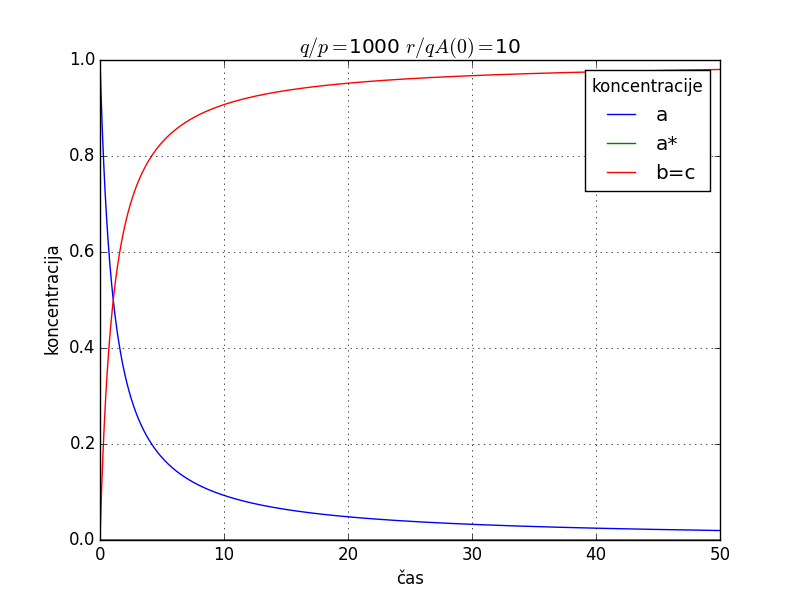
\includegraphics[scale=0.4]{slike/q_p_1000_r_qA(0)_10.png}
\hspace{\fill}
\end{flushleft}
\end{minipage}
\begin{minipage}[t]{0.5\paperwidth}
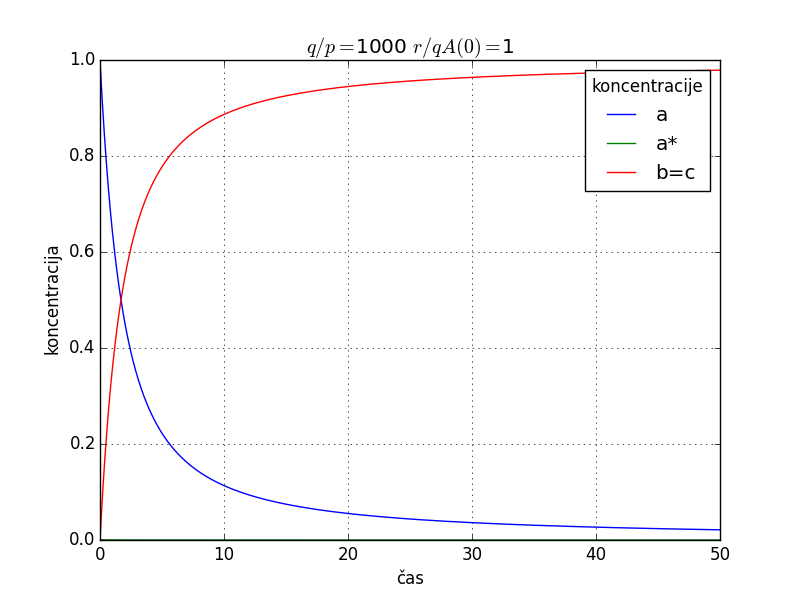
\includegraphics[scale=0.4]{slike/q_p_1000_r_qA(0)_1.png}
\end{minipage}%
}
\noindent\makebox[\textwidth][l]{%
\hspace{-\dimexpr\oddsidemargin+1in}%

\begin{minipage}[t]{0.5\paperwidth}
\begin{flushleft}

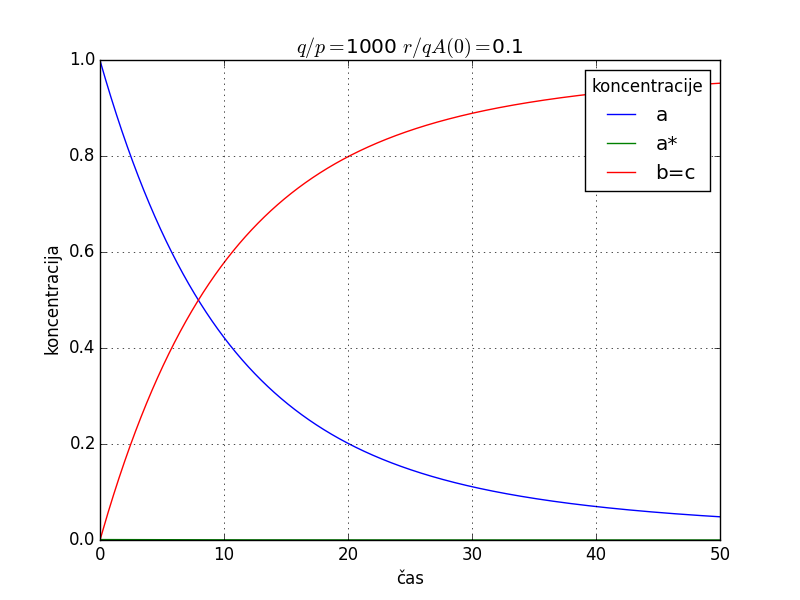
\includegraphics[scale=0.4]{slike/q_p_1000_r_qA(0)_0_1.png}
\hspace{\fill}
\end{flushleft}
\end{minipage}
\begin{minipage}[t]{0.5\paperwidth}
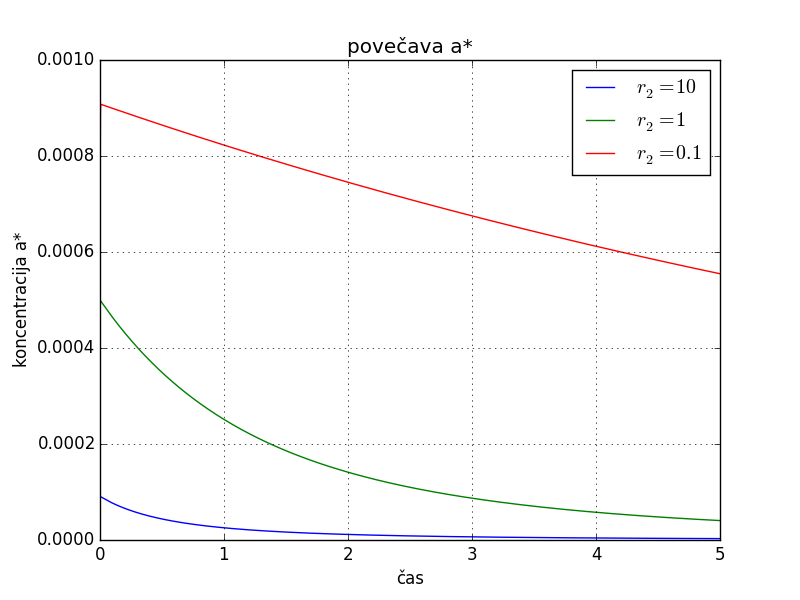
\includegraphics[scale=0.4]{slike/povecaca_binarana.png}
\end{minipage}%
}
\caption{Primeri rešitev za nekaj različnih parametrov $r_2$.}
\end{figure}
\pagebreak


\subsection{Aproksimacija stacionarnega stanja}
V zgornjih treh primerih opazimo, da je koncentracija vzbujenega stanja $a^*$ tri velikostne razrede manjša, kot koncentracija $a$, $b$, ter $c$ snovi. To je posledica, saj smo določili parametru veliko vrednost $r_1=1000$, oz. snov rajši razpade v osnovno stanje. S približno isto hitrostjo, kot nastaja stanje $a^*$, iz tega stanja razpada v končno stanje $b$, $c$. Koncentracija tega s časom narašča, saj se ta produkt nabira v sistemu. Večji je $r2$, hitreje se približuje proti končni vrednosti. To je posledica, ker se v parametru $r_2$ skriva razmerje med $r$ in $q$. Kot omenjeno, je koncentracija $a^*$ nekaj velikostnih razredov manjša, ter se tudi počasi spreminja s časov. Sedaj predpostavimo, da je $\dot{a^*}=0$. Enačbe \ref{eq-binarne-brezdim} se sedaj zapišejo:

\begin{equation}
\label{eq-binarne-stacio-brezdim}
\begin{aligned}
& \dot{a}= - \frac{r_2 a^2}{r_2 + a}\\
&  a^* = \frac{a^2}{r_1 (a+ r_2)}
\end{aligned}
\end{equation}

Primerjajmo aproksimacijo stacionarnega stanja z analitično rešitvijo. Ker nas zanima, kako dober je približek si oglejmo absolutno vrednost razlike med analitično rešitvijo in približkov stacionarnega stanja.
\begin{figure}[h]
\noindent\makebox[\textwidth][l]{%
\hspace{-\dimexpr\oddsidemargin+1in}%

\begin{minipage}[t]{0.5\paperwidth}
\begin{flushleft}
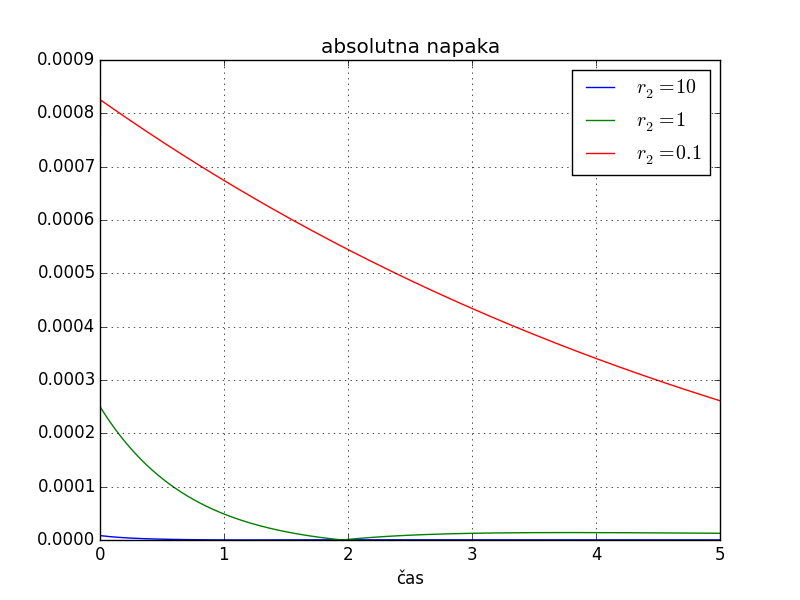
\includegraphics[scale=0.5]{slike/absolutna_napaka.png}
\hspace{\fill}
\end{flushleft}
\end{minipage}
\begin{minipage}[t]{0.5\paperwidth}
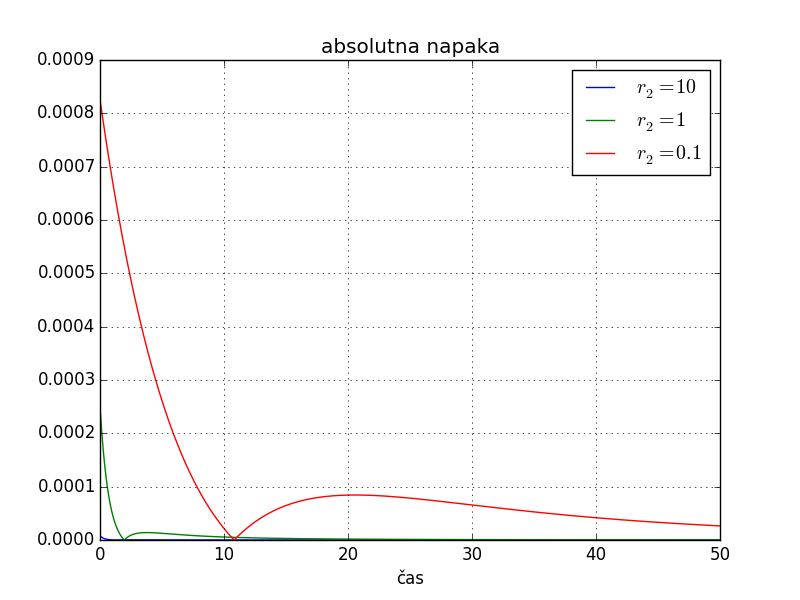
\includegraphics[scale=0.5]{slike/absolutna_napak_500000.png}
\end{minipage}%
}

\caption{Absolutna vrednost razlike med analitično rešitvijo in aproksimacijo stacionarnega stanja.}
\end{figure}

Opazimo, da približek dobro deluje za večje čase, saj se napaka opazi čele na tretjem decimalnem mestu.

\section{Reakcija vodikovega bromida}
Imamo kemijsko reakcijo ${\rm H}_2+{\rm Br}_2\rightleftharpoons 2{\rm HBr}$, ki jo po stopnjah zapišemo:

  \begin{align*}
    {\rm Br}_2 & \mathop{\rightleftharpoons}_{q}^{p} 2{\rm Br},\\
    {\rm Br}+{\rm H}_2 &\mathop{\rightleftharpoons}_{s}^{r} {\rm H Br}+{\rm H},\\
    {\rm H}+{\rm Br}_2 &\mathop{\rightarrow}_{t} {\rm H Br}+{\rm Br}.
  \end{align*}
Sistem opišemo s naslednjimi diferencialnimi enačbami:

\begin{equation}
\begin{aligned}
\dot{x}=& -rvx + szu \\
\dot{y}=& -py + q v^2 -t u y \\
\dot{z}=& -s z u + r x v -t u y \\
\dot{u}=0=& r v x - s z u - t u y \\
\dot{v}=0=& -q v^2 + p y -r v x + t u y + s z u
\end{aligned}
\end{equation}
kjer so $x$, $y$, $z$, koncentracije $H_2$, $Br_2$, $HBr$ ter $u$, $v$ koncentraciji $H$, $Br$. V zgornji enačbi smo že upoštevali aproksimacijo stacionarnega stanja, ko smo hitrost spremembe koncentraciji $u$, $v$, enačili z nič. Ko rešimo sistem enačb, dobimo naslednje rešitve za hitrosti osnovnih elementov reakcije:
\begin{equation}
\begin{aligned}
\dot{x}= \dot{y}=& - \sqrt{\frac{p}{q}}  \frac{t r }{s } \frac{x \sqrt{y}}{\frac{z}{y}+ \frac{t}{s}} \\
\dot{z}=& -2 \dot{x}
\end{aligned}
\end{equation}
Če primerjamo zgornjo enačbo z analitično rešitvijo:
\begin{equation*}
\dot{z}=\frac{k x y^{1/2}}{m+\frac{z}{y}}
\end{equation*}
vidimo, da imata parametra naslednji vrednosti $k=2\sqrt{\frac{p}{q}}  \frac{t r }{s }$, $m=\frac{t}{s}$.\\
Oglejmo si nekaj rešitev, pri $m=2.5$, $k=1$. Začetna vrednost koncentracije: $[HBr]=0$, razmerje med začetno koncentracijo označimo $\alpha=\frac{[H_2]}{Br_2}$. Skupna koncentracija je $[HBr]+[H_2]+[Br_2]=1$.

\begin{figure}[h]
\noindent\makebox[\textwidth][l]{%
\hspace{-\dimexpr\oddsidemargin+1in}%

\begin{minipage}[t]{0.5\paperwidth}
\begin{flushleft}
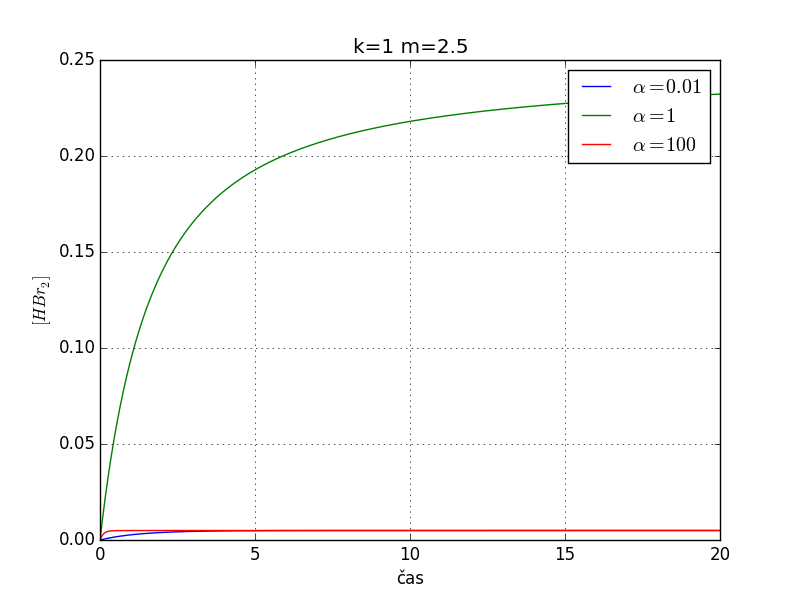
\includegraphics[scale=0.4]{slike/prva-osnovna.png}
\hspace{\fill}
\end{flushleft}
\end{minipage}
\begin{minipage}[t]{0.5\paperwidth}
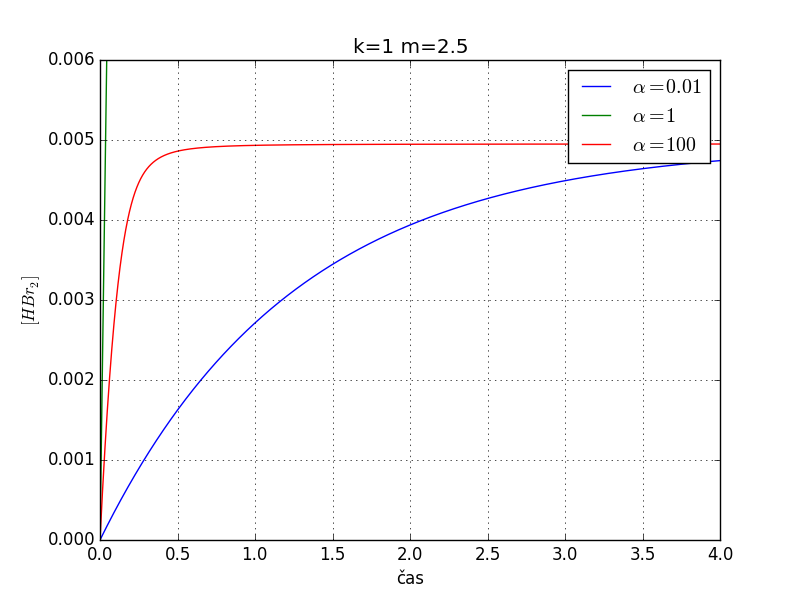
\includegraphics[scale=0.4]{slike/prva-osnovna_povecava.png}
\end{minipage}%
}

\caption{Primeri rešitev za $m=2.5$, $k=1$, pri različnih začetnih razmerjih. Na desni povečava levega grafa.}
\end{figure}
Vidimo, da pri enaki začetni koncentraciji vodika in broma, dobimo največ $[HBr]$. V primeru, da želimo čim hitrejšo stabilizacijo sistema, je bolje imeti več vodika, kot broma. Kako na sistem vplivamo, če na začetku dodajamo $[HBr]$?

\begin{figure}[h]
\noindent\makebox[\textwidth][l]{%
\hspace{-\dimexpr\oddsidemargin+1in}%

\begin{minipage}[t]{0.5\paperwidth}
\begin{flushleft}
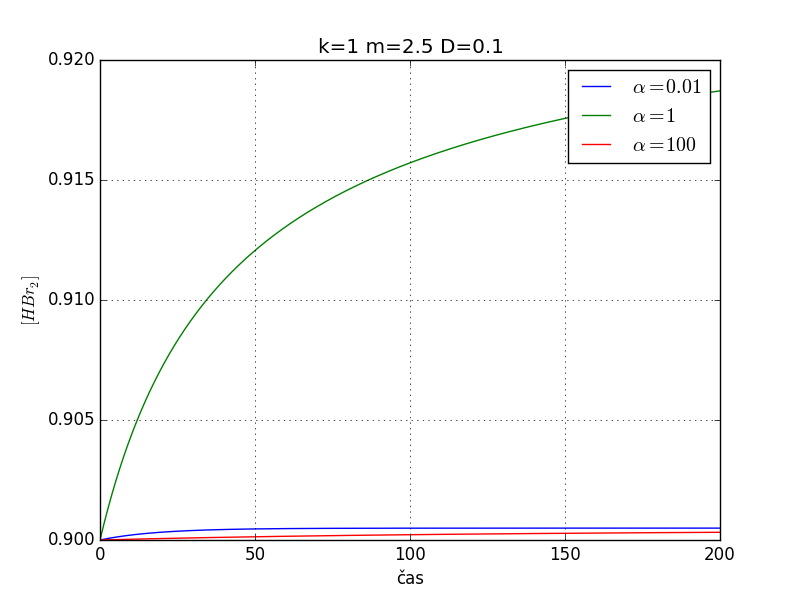
\includegraphics[scale=0.4]{slike/druga_druga_D_0_1_png}
\hspace{\fill}
\end{flushleft}
\end{minipage}
\begin{minipage}[t]{0.5\paperwidth}
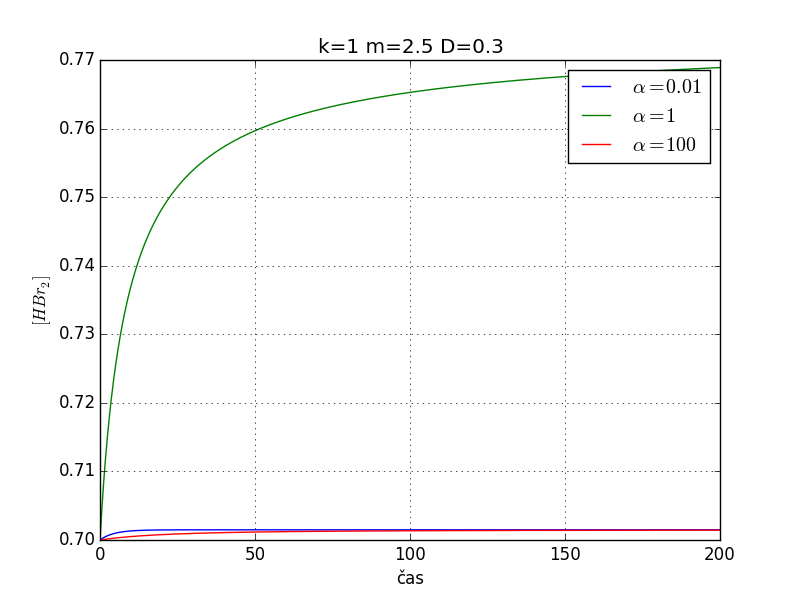
\includegraphics[scale=0.4]{slike/druga_druga_D_0_3_png}
\end{minipage}%
}
\noindent\makebox[\textwidth][l]{%
\hspace{-\dimexpr\oddsidemargin+1in}%

\begin{minipage}[t]{0.5\paperwidth}
\begin{flushleft}

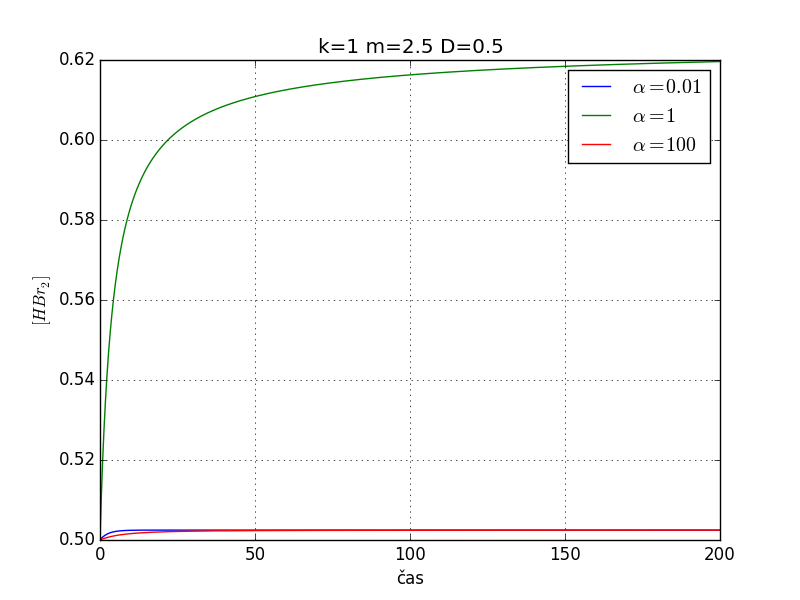
\includegraphics[scale=0.4]{slike/druga_druga_D_0_5_png}
\hspace{\fill}
\end{flushleft}
\end{minipage}
\begin{minipage}[t]{0.5\paperwidth}
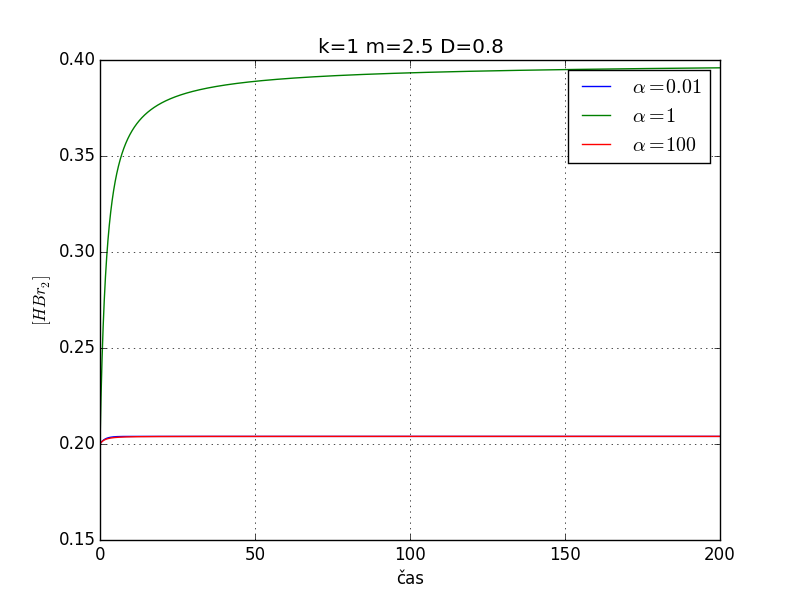
\includegraphics[scale=0.4]{slike/druga_druga_D_0_8_png}
\end{minipage}%
}
\caption{Primeri rešitev za različne začetne koncentracije $[HBr]$. V vsakem primeru se koncentracija poveča.}
\end{figure}

\pagebreak
\section{Kemijska ura}
Kemijske ure so reakcije, ki stečejo s predvidljivim in
  ponavadi ostrim časovnim zamikom. Primer take reakcije je
  \emph{jodova ura}, ki v eni izmed izvedb temelji na ravnotežju
  naslednjih reakcij:
\begin{align*}
  \sul_2\oxi_8^{2-}+2\jod^- &\rightarrow \jod_2+2\sul\oxi_4^{2-},\\
  2\sul_2\oxi_3^{2-}+\jod_2 &\rightarrow2\jod^- + \sul_4 \oxi_6^{2-}.
\end{align*}
Druga reakcija je bistveno hitrejša od prve, mehanizem merjenja časa
pa je enakomerno porabljanje tiosulfata $\sul_2\oxi_3^{2-}$. Če je
persulfat $\sul_2\oxi_8^{2-}$ v prebitku, lahko za aktivne
spremenljivke vzamemo le $[\jod^-]$, $[\jod_2]$ in $[\sul_2
  \oxi_3^{2-}]$.%, sicer pa moramo upoštevati tudi porabljanje persulfata.

Obe zgornji reakciji sta v resnici sosledji dveh binarnih reakcij preko
kratkoživega prehodnega stanja. Prva reakcija je sestavljena iz stopenj
\begin{align*}
  \sul_2\oxi_8^{2-}+\jod^-&\xrightarrow{\makebox[1cm][c]{\text{\tiny počasi}}} \jod\sul_2\oxi_8^{3-},\\
  \jod\sul_2\oxi_8^{3-}+\jod^-&\xrightarrow{\makebox[1cm][c]{\text{\tiny hitro}}} \jod_2+2\sul\oxi_4^{2-},
\end{align*}
druga pa iz stopenj
\begin{align*}
 \sul_2\oxi_3^{2-}+\jod_2\xrightarrow{\makebox[1cm][c]{\text{\tiny počasi}}}\jod\sul_2\oxi_3^{-}+\jod^-,\\
 \jod\sul_2\oxi_3^-+\sul_2\oxi_3^{2-}\xrightarrow{\makebox[1cm][c]{\text{\tiny hitro}}}\jod^-+\sul_4\oxi_6^{2-}.
\end{align*}
Ta sistem, po upoštevanju približka stacionarnega stanja, ter uvedbi brezdimenzijskih količin, prepišemo v enačbe:
\begin{equation}
\begin{aligned}
\dot{x}=& -2 x w + 2 \lambda y z \\
\dot{y}=& x w - \lambda y z \\
\dot{z}=& -2 \lambda y z \\
\dot{w}=& -x w
\end{aligned}
\end{equation}
Spremenljivke $x$, $y$, $z$ ter $w$ so koncentracije $[I^-]$,$[I_2]$,$[S_2 O_3^{2-}]$ in $[S_2 O_8^{2-}]$. Parameter $\lambda$, pa je razmerje hitrosti med počasnima reakcijama $\frac{s_2}{s_1}$.
Poglejmo si nekaj rešitev:

\begin{figure}[h]
\noindent\makebox[\textwidth][l]{%
\hspace{-\dimexpr\oddsidemargin+1in}%

\begin{minipage}[t]{0.5\paperwidth}
\begin{flushleft}
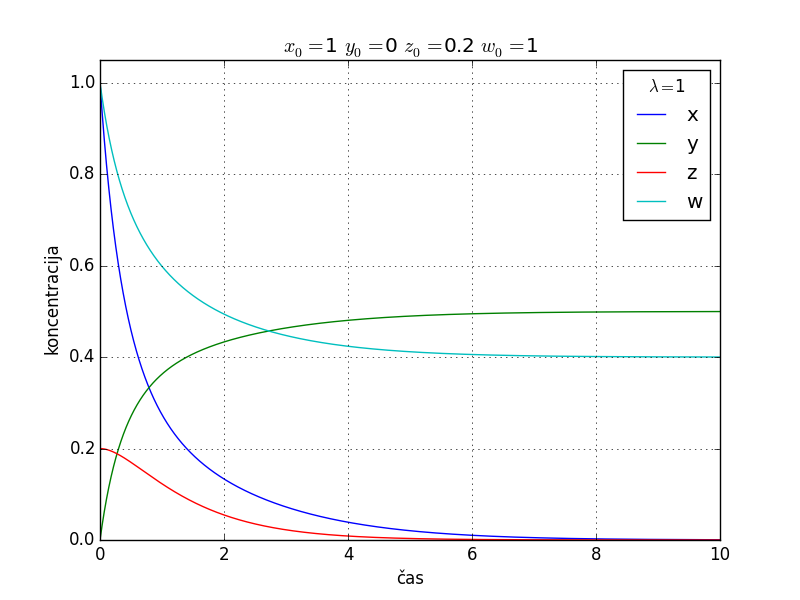
\includegraphics[scale=0.4]{slike/110_21.png}
\hspace{\fill}
\end{flushleft}
\end{minipage}
\begin{minipage}[t]{0.5\paperwidth}
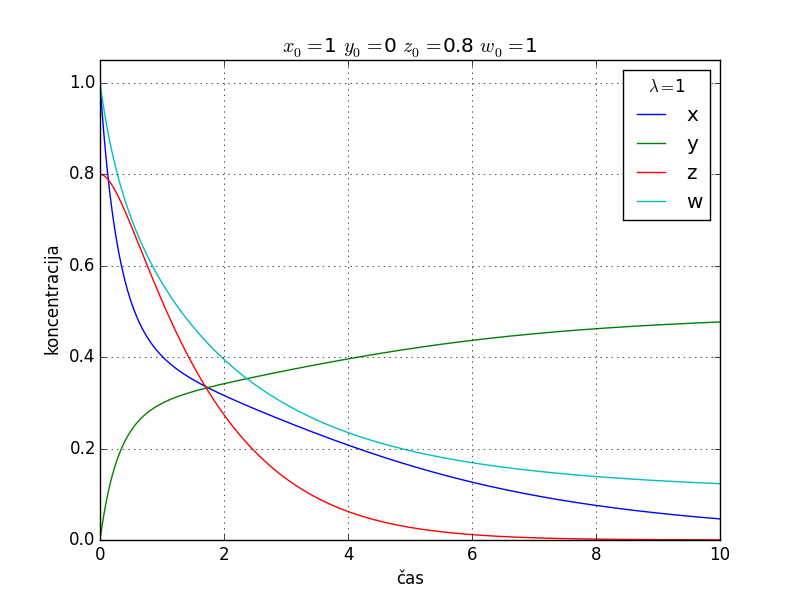
\includegraphics[scale=0.4]{slike/110_81.png}
\end{minipage}%
}
\noindent\makebox[\textwidth][l]{%
\hspace{-\dimexpr\oddsidemargin+1in}%

\begin{minipage}[t]{0.5\paperwidth}
\begin{flushleft}

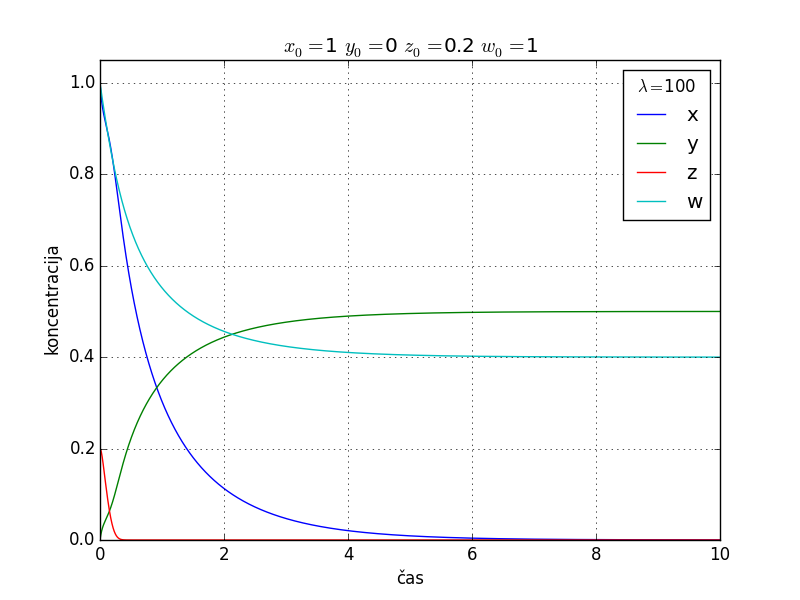
\includegraphics[scale=0.4]{slike/110_2100.png}
\hspace{\fill}
\end{flushleft}
\end{minipage}
\begin{minipage}[t]{0.5\paperwidth}
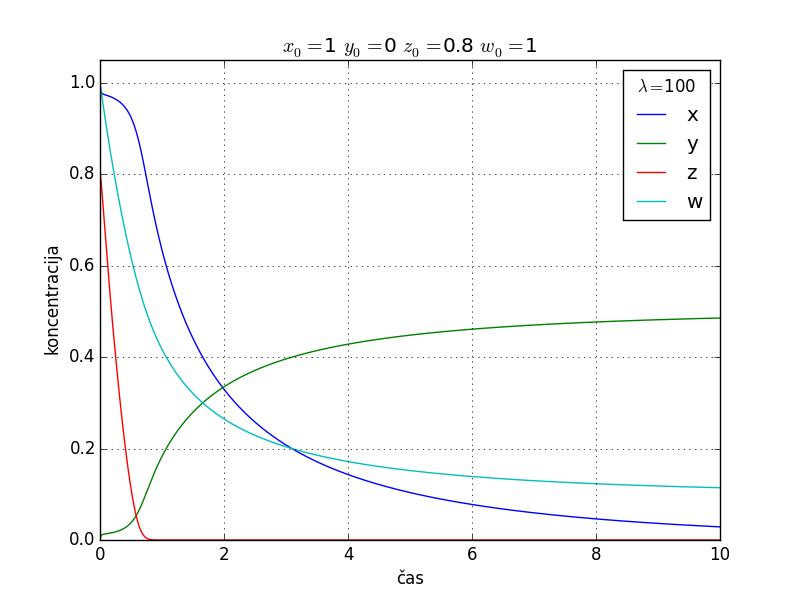
\includegraphics[scale=0.4]{slike/110_8100.png}
\end{minipage}%
}
\caption{Primeri rešitev za različne začetne koncentracije in različne vrednosti parametra $\lambda$. Opazimo, da pri večji vrednosti $\lambda$ koncentracije hitreje konvergirajo proti stacionarnim vrednostim. S spreminjanjem začetne koncentracije $S_2 O_8^{2-}$ spreminjamo stacionarne vrednosti ostalim snovem.}
\end{figure}



\end{document}
